\input{../Preambulos/preambulo_materiales}
\usepackage{chemformula}
\title{Física Estadística\vspace{-3ex}}
\author{M. en C. Gustavo Contreras Mayén}
\date{ }

\begin{document}

\vspace{-4cm}
\maketitle
\fontsize{14}{14}\selectfont
\tableofcontents
\newpage

\section{Física Estadística.}
\subsection{Base estadística de la termodinámica.}

%Ref. Pathria.

En los anales de la física térmica, la década de 1850 marca una época muy definida. En ese momento, la ciencia de la termodinámica, que surgió esencialmente de un estudio experimental del comportamiento macroscópico de los sistemas físicos, se había convertido, a través del trabajo de Carnot, Joule, Clausius y Kelvin, en una disciplina física segura y estable. Se encontró que las conclusiones teóricas que se derivan de las dos primeras leyes de la termodinámica concuerdan muy bien con los resultados experimentales correspondientes. Al mismo tiempo, la teoría cinética de los gases, cuyo objetivo es explicar el comportamiento macroscópico de los sistemas gaseosos en términos del movimiento de sus moléculas y que hasta ahora había prosperado más en la especulación que en el cálculo, comenzó a emerger como una teoría matemática real. Sus éxitos iniciales fueron deslumbrantes; sin embargo, no se pudo establecer un contacto real con la termodinámica hasta alrededor de 1872, cuando Boltzmann desarrolló su teorema H y, por lo tanto, estableció una conexión directa entre la entropía por un lado y la dinámica molecular por el otro. Casi simultáneamente, la teoría convencional (cinética) comenzó a dar paso a su sucesora más sofisticada: la teoría del conjunto. El poder de las técnicas que finalmente surgieron redujeron la termodinámica al estatus de una consecuencia \enquote{esencial} del encuentro de las estadísticas y la mecánica de las moléculas que constituyen un sistema físico dado. Entonces fue natural dar al formalismo resultante el nombre de \emph{mecánica estadística}.
\par
Como preparación para el desarrollo de la teoría formal, comenzamos con algunas consideraciones generales sobre la naturaleza estadística de un sistema macroscópico. Estas consideraciones proporcionarán la base para una interpretación estadística de la termodinámica. Cabe mencionar aquí que, a menos que se haga una afirmación en contrario, se supone que el sistema en estudio se encuentra en uno de sus estados de equilibrio.

\subsection{Estados macro y microscópicos.}

Consideramos un sistema físico compuesto de $N$ partículas idénticas confinadas a un espacio de volumen $V$. En un caso típico, $N$ sería un número extremadamente grande, generalmente del orden de $\num{d23}$. En vista de esto, es habitual realizar análisis en el llamado \emph{límite termodinámico}, a saber, $N \to \infty$, $V \to \infty$ (tal que la relación $N / V$, que representa la \emph{densidad de partículas} $n$, permanece fija en un valor preasignado). En este límite, las \emph{propiedades extensivas} del sistema se vuelven directamente proporcionales al tamaño del sistema (es decir, proporcionales a $N$ o a $V$ ), mientras que las \emph{propiedades intensivas} se vuelven independientes del mismo; la densidad de partículas, por supuesto, sigue siendo un parámetro importante para todas las propiedades físicas del sistema.
\par
A continuación consideramos la energía total $E$ del sistema. Si se pudiera considerar que las partículas que componen el sistema no interactúan, la energía total $E$ sería igual a la suma de las energías $\varepsilon_{i}$ de las partículas individuales:
\begin{align}
E = \nsum_{i} n_{i} \, \varepsilon_{i}
\label{eq:ecuacion_01_01}
\end{align}
donde $n_{i}$ indica el número de partículas cada una con energía $\varepsilon_{i}$. Se entiende claramente que:
\begin{align}
N = \nsum_{i} n_{i}
\label{eq:ecuacion_02_02}
\end{align}
De acuerdo con la mecánica cuántica, las energías de una sola partícula $\varepsilon_{i}$ son discretas y sus valores dependen crucialmente del volumen $V$ al que están confinadas las partículas. En consecuencia, los valores posibles de la energía total $E$ también son discretos. Sin embargo, para grandes $V$, el espaciamiento de los diferentes valores de energía es tan pequeño en comparación con la energía total del sistema que el parámetro $E$ bien podría considerarse como una \emph{variable continua}. Esto sería cierto incluso si las partículas interactuaran entre sí; por supuesto, en ese caso la energía total $E$ no puede escribirse en la forma de la ec. (\ref{eq:ecuacion_01_01}).
\par
La especificación de los valores reales de los parámetros $N$, $V$ y $E$ define un \emph{macroestado} del sistema dado.
\par
A nivel molecular, sin embargo, todavía existe un gran número de posibilidades porque en ese nivel habrá \emph{en general} un gran número de formas diferentes en las que se puede realizar el macroestado $(N, V, E)$ del sistema dado. En el caso de un sistema que no interactúa, dado que la energía total $E$ consiste en una simple suma de las $N$ energías $\varepsilon_{i}$ de una sola partícula, obviamente habrá un gran número de formas diferentes en las que se puede elegir el $\varepsilon_{i}$ individual para hacer que la energía total sea igual a $E$. En otras palabras, habrá un gran número de formas diferentes en las que la energía total $E$ del sistema puede distribuirse entre las $N$ partículas que lo constituyen. Cada una de estas formas (diferentes) especifica un \emph{microestado}, o \emph{complexión}, del sistema dado. En general, los diversos microestados, o complexiones, de un sistema dado pueden identificarse con las soluciones independientes $\psi (\vb{r}_{1}, \ldots, \vb{r}{N})$ de la ecuación de Schrödinger del sistema, correspondiente al valor propio $E$ del Hamiltoniano relevante. En cualquier caso, a un macroestado dado del sistema le corresponde en general un gran número de microestados y parece natural suponer, cuando no hay otras restricciones, que en cualquier momento $t$ es igualmente probable que el sistema se encuentre en cualquiera de estos microestados. Esta suposición forma la columna vertebral de nuestro formalismo y generalmente se la conoce como el postulado de \enquote{probabilidades iguales \emph{a priori}} para todos los microestados consistentes con un macroestado dado.
\par
El número real de todos los microestados posibles será, por supuesto, una función de $N$, $V$ y $E$, puede denotarse con el símbolo $\Omega (N, V, E)$; la dependencia de $V$ surge porque los posibles valores $\varepsilon_{i}$ de la energía $\varepsilon$ de una sola partícula son en sí mismos una función de este parámetro. Sorprendentemente, es a partir de la magnitud del número $\Omega$, y de su dependencia de los parámetros $N$, $V$ y $E$, que se puede derivar la termodinámica completa del sistema dado.
\par
No nos detendremos aquí para discutir las formas en que se puede calcular el número $\Omega (N, V, E)$; lo haremos sólo después de que hayamos desarrollado nuestras consideraciones lo suficiente como para que podamos llevar a cabo más derivaciones a partir de ellas. Primero tenemos que descubrir la manera en que este número se relaciona con cualquiera de las principales cantidades termodinámicas. Para hacer esto, consideramos el problema del \enquote{contacto térmico} entre dos sistemas físicos dados, con la esperanza de que esta consideración revele la verdadera naturaleza del número $\Omega$.

\subsection{Significado físico del número \texorpdfstring{$\Omega (N, V, E)$}{O (N,V,E).}}

Consideremos dos sistemas físicos, $A_{1}$ y $A_{2}$, que están en equilibrio por separado, como se presenta en la figura (\ref{fig:figura_01_01}).
\begin{figure}[H]
    \centering
    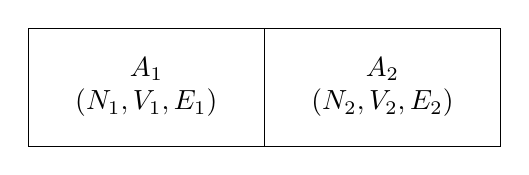
\begin{tikzpicture}
        \draw [align=center] (0, 0) rectangle (3, 1.5) node [pos=0.5] {$A_{1}$ \\ $(N_{1}, V_{1}, E_{1})$};
        \draw [align=center] (3, 0) rectangle (6, 1.5) node [pos=0.5] {$A_{2}$ \\ $(N_{2}, V_{2}, E_{2})$};
    \end{tikzpicture}
    \caption{Dos sistemas físicos que se ponen en contacto térmico.}
    \label{fig:figura_01_01}
\end{figure}
Sea el macroestado de $A_{1}$ representado por los parámetros $N_{1}, V_{1}$ y $E_{1}$ de manera que tenga $\Omega_{1} (N_{1}, V_{1}, E_{1})$ microestados posibles, y sea el macroestado de $A_{2}$ representado por los parámetros $N_{2}, V_{2}$ y $E_{2}$ de manera que tiene $\Omega_{2} (N_{2}, V_{2}, E_{2})$ posibles microestados. La forma matemática de la función $\Omega_{1}$ puede no ser la misma que la de la función $\Omega_{2}$, porque eso depende en última instancia de la naturaleza del sistema. Por supuesto, creemos que todas las propiedades termodinámicas de los sistemas $A_{1}$ y $A_{2}$ pueden ser derivados de las funciones $\Omega_{1} (N_{1}, V_{1}, E_{1})$ y $\Omega_{2} (N_{2}, V_{2}, E_{2})$, respectivamente.
\par
Ahora ponemos los dos sistemas en contacto térmico entre sí, permitiendo así la posibilidad de intercambio de energía entre los dos; esto se puede hacer deslizando una pared conductora y quitando la impermeable. Para simplificar, los dos sistemas todavía están separados por una pared rígida e impenetrable, de modo que los respectivos volúmenes $V_{1}$ y $V_{2}$ y los respectivos números de partículas $N_{1}$ y $N_{2}$ permanecen fijos. Las energías $E_{1}$ y $E_{2}$, sin embargo, se vuelven variables y la única condición que restringe su variación es:
\begin{align}
E^{(0)} = E_{1} + E_{2} = \text{constante}
\label{eq:ecuacion_02_01}
\end{align}
Aquí, $E^{(0)}$ indica la energía del sistema compuesto $A^{(0)} (\equiv A_{1} + A_{2})$; se desprecia la energía de interacción entre $A_{1}$ y $A_{2}$, si la hay. Ahora, en cualquier momento $t$, es igualmente probable que el subsistema $A_{1}$ se encuentre en cualquiera de los microestados $\Omega_{1} (E_{1})$, mientras que es igualmente probable que el subsistema $A_{2}$ se encuentre en cualquiera de los microestados $\Omega_{2} (E_{2})$; por lo tanto, es igualmente probable que el sistema compuesto $A^{(0)}$ esté en cualquiera de los:
\begin{align}
\Omega_{1} (E_{1}) \, \Omega_{2} (E_{2}) = \Omega_{1} (E_{1}) \, \Omega_{2} (E^{(0)} - E_{1}) = \Omega^{(0)} (E^{(0)}, E_{1})
\label{eq:ecuacion_02_02}
\end{align}
microestados. Claramente, el número $\Omega^{(0)}$ en sí mismo varía con $E_{1}$. Surge ahora la siguiente pregunta: ¿a qué valor de $E_{1}$ estará en equilibrio el sistema compuesto? En otras palabras, ¿hasta dónde llegará el intercambio de energía para que los subsistemas $A_{1}$ y $A_{2}$ alcancen un equilibrio mutuo?
\par
Afirmamos que esto sucederá en ese valor de $E_{1}$ que maximiza el número $\Omega^{(0)} (E^{(0)}, E_{1})$. La filosofía detrás de esta afirmación es que un sistema físico, abandonado a sí mismo, procede naturalmente en una dirección que le permite asumir un número cada vez mayor de microestados hasta que finalmente se establece en un macroestado que ofrece el \emph{mayor número posible} de microestados. Estadísticamente hablando, consideramos un macroestado con un mayor número de microestados como un estado más probable, y el que tiene un mayor número de microestados como el más probable. Estudios detallados muestran que, para un sistema típico, el número de microestados pertenecientes a cualquier macroestado que se desvía aunque sea ligeramente del más probable es \enquote{órdenes de magnitud} menor que el número perteneciente a este último. Por tanto, el estado más probable de un sistema es el macroestado en el que el sistema pasa una fracción abrumadoramente grande de su tiempo. Entonces es natural identificar este estado con el estado de \emph{equilibrio} del sistema.
\par
Denotando el valor de equilibrio de $E_{1}$ por $\bar{E}_{1}$ (y el de $E_{2}$ por $\bar{E}_{2})$, obtenemos, al maximizar $\Omega^{(0)}$:
\begin{align*}
\left( \pdv{\Omega_{1} (E_{1})}{E_{1}} \right) \eval_{E_{1} = \bar{E}_{1}} \, \Omega_{2} (\bar{E}_{2}) + \Omega_{1} (\bar{E}_{1}) \, \left( \pdv{\Omega_{2} (E_{2})}{E_{2}} \right) \eval_{E_{2} = \bar{E}_{2}} \cdot \pdv{E_{2}}{E_{1}} = 0
\end{align*}
Ya que $\pdv*{E_{2}}{E_{1}} = -1$, ver la ec. (\ref{eq:ecuacion_02_01}), la condición anterior se puede escribir como:
\begin{align*}
\left( \pdv{\ln \Omega_{1} (E_{1})}{E_{1}} \right) \eval_{E_{1} = \bar{E}_{1}} = \left( \pdv{\ln \Omega_{2} (E_{2})}{E_{2}} \right) \eval_{E_{2} = \bar{E}_{2}}
\end{align*}
Así, nuestra condición de equilibrio se reduce a la igualdad de los parámetros $\beta_{1}$ y $\beta_{2}$ de los subsistemas $A_{1}$ y $A_{2}$, respectivamente, donde $\beta$ está definido por:
\begin{align}
\beta = \left( \pdv{\ln \Omega (N, V, E)}{E} \right)_{N, V, E = \bar{E}}
\label{eq:ecuacion_02_03}
\end{align}
Así encontramos que cuando dos sistemas físicos se ponen en contacto térmico, lo que permite un intercambio de energía entre ellos, este intercambio continúa \emph{hasta} que se alcanzan los valores de equilibrio $\bar{E}_{1}$ y $\bar{E}_{2}$ de las variables $E_{1}$ y $E_{2}$. Una vez que se alcanzan estos valores, no hay más intercambio neto de energía entre los dos sistemas; se dice entonces que los sistemas han alcanzado un estado de equilibrio térmico. De acuerdo con nuestro análisis, esto sucede solo cuando los valores respectivos del parámetro $\beta$, es decir, $\beta_{1}$ y $\beta_{2}$, se igualan. Entonces es natural esperar que el parámetro $\beta$ esté relacionado de alguna manera con la \emph{temperatura termodinámica} $T$ de un sistema dado. Para determinar esta relación, recordamos la fórmula termodinámica:
\begin{align}
\left( \pdv{S}{E} \right)_{N, V} = \dfrac{1}{T}
\label{eq:ecuacion_02_04}
\end{align}
donde $S$ es la entropía del sistema en cuestión. Comparando las ecuaciones (\ref{eq:ecuacion_02_03}) y (\ref{eq:ecuacion_02_04}), concluimos que existe una íntima relación entre la cantidad termodinámica $S$ y la cantidad estadística $\Omega$; podemos, de hecho, escribir para cualquier sistema físico
\begin{align}
\dfrac{\Delta S}{\Delta (\ln \Omega)} = \dfrac{1}{\beta \, T} = \text{constante}
\label{eq:ecuacion_02_05} 
\end{align}
Esta correspondencia fue establecida por primera vez por Boltzmann, quien también creía que, dado que la relación entre el enfoque termodinámico y el enfoque estadístico parece tener un carácter fundamental, la constante que aparece en la ec. (\ref{eq:ecuacion_02_05}) debe ser una \emph{constante universal}. Fue Planck quien primero escribió la fórmula explícita:
\begin{align}
S = k \, \ln \Omega
\label{eq:ecuacion_02_06}
\end{align}

\end{document}